\begin{chapter}{\label{cha:intro}Introduction}

  \section{\label{sec:jointintro}Background to the joint modelling of survival and longitudinal data}
  In many areas of health research, collection of (potentially many) repeated measurements which are censored by a terminal event are commonplace. Interest then falls on the longitudinal trajectories, risk of event occurrence, and the relationship between the two. The longitudinal process is endogenous and time-dependent if thought to be related to the risk of event occurrence, but simply including the process in de facto modelling approaches is inappropriate \citep{Prentice1982, Kalbfleisch2002, Sweeting2011}.
  
  When the longitudinal outcome and the time-to-event of interest are related, the modelling process must consider dropouts as non-random. Incorporation of the survival information into the longitudinal process has an equivalence to taking into account the effect of an informative missing data process \citep{Sweeting2011}. Conversely, incorporation of the longitudinal information into the survival process improves the fit of regression (\ie reducing biases arising from separate model fits) and importantly provides inference on the relation between the event time and the longitudinal process \citep{Wulfsohn97,Sweeting2011}.

  Joint modelling arose as a solution to problems arising from HIV/AIDS research in the first instance. Namely, it allowed researchers to \textit{simultaneously} answer three questions of scientific interest:
  \begin{enumerate}
      \item How do the biomarker(s) of interest evolve through time and differ in terms of the other covariates collected at baseline (\eg drug allocation, sex)?
      \item How does the hazard for the event of interest evolve through time and differ in terms of the other covariates collected at baseline?
      \item How is this hazard affected by underlying values of the biomarker(s) of interest?
  \end{enumerate}
  At heart then, a joint model consists of at least two sub-models with some shared random effects that are combined into one larger meta-model by linking these random effects. Commonly adopted sub-models are a linear mixed effects model (LMM, \citet{LairdWare1982}), and a Cox proportional hazards (PH) model \citep{Cox1972} for the longitudinal and survival components respectively.

  Early efforts however were na\"{i}ve in their implementation, simply including the biomarker as a time-dependent covariate in the PH model. One such example of this approach being \citet{Andersen1982}, producing estimates for association which were underestimated \citep{Prentice1982, Sweeting2011}. Additionally, such an approach does not model the longitudinal profile itself, which was one research question we sought to answer.

  Next saw so-called `two-stage' models which provided improvement over the preceding na\"{i}ve approach. Essentially a `two-stage' model extracts the random effects from the LMM and models these as time-varying covariates in the PH model. Both \citet{Tsiatis1995} and \citet{DeGruttola1994} used this approach along with an application to aforementioned HIV/AIDS data, albeit with slight reparameterisation of the survival process in the latter example. This modelling approach is relatively easy to implement, and reduced the bias obtained in parameter estimates in comparison with na\"{i}ve methods \citep{Dafni1998}.

  Joint models, as they appear in this thesis, then arose in \citet{Wulfsohn97}. Often seen as the  `first' joint modelling paper, it was in fact predated by efforts conducted under Bayesian hierarchical frameworks, for instance \citet{Berzuini1996} and \citet{Faucett1996}. Given these Bayesian efforts predated standard software such as \tt{WinBUGS} \citep{Winbugs-manual}, or because clinicians typically operate under the frequentist paradigm, these are perhaps secondary to the seminal \citet{Wulfsohn97} in retrospect.

  \citet{Wulfsohn97} introduced the joint modelling of longitudinal and time-to-event data using maximum likelihood estimation via the Expectation Maximisation (EM) algorithm \citep{Dempster77}. Their approach 
  accounting for the informative dropout process and incorporated the observed survival information in modelling the longitudinal process; essentially the available information is most efficiently used \citep{JMOverview}. Justifications for joint models over the na\"{i}ve and `two-stage' models abound in literature, two examples showcasing the reduced bias obtained from the joint model are \citet{Ibrahim2010} and \citet{Sweeting2011}, the latter also highlighting that joint models perform well despite model misspecification.

  \section{Evolution of joint models}\label{sec:intro-evolution-parent}
  %\rmtoc
  % Random effects structure -->
  \subsection{Random effects specification}\label{sec:intro-evolution-REs}
  \citet{Wulfsohn97} demonstrated their approach using a simplified model containing only the random effects in both the longitudinal and survival sub-models in an application to the HIV/AIDS data which spurred its initial materialisation. Perhaps acting as something of a `proof of concept', it neatly set the stage for extensions to the basic model presented therein. \citet{Tsiatis1995}, \citet{Faucett1996}, \citet{Bycott1998}, \citet{Dafni1998}, and \citet{Wulfsohn97} all assumed bivariate Gaussian random effects in the form of a random intercept and slope structure when approaching the joint model. In later literature especially, the random effects have become increasingly complex, with use of \eg spline terms \citep{Martins2022, Rustand2023}. Elsewhere, \citet{Henderson2000} added complexity to the random effects specification by introducing a stationary Gaussian process, similarly carried out in \citet{Xu2001} using Bayesian methods. Finally, \citet{Wang2001} provide an example of using a non-stationary Gaussian process. 

  \subsection{Alternative sub-models}\label{sec:intro-evolution-glmm}
  Joint models do not solely rely on the previously mentioned linear mixed and Cox proportional hazards models. Two (not necessarily exclusive) ways have emerged in the literature.

  The first replaces the PH model with a generalised linear model (GLM). For example, if occurrence of an event of interest is more important than the \textit{timing} of it, then the PH model is replaced by a binary (i.e. logistic) sub-model. Examples include primary endpoints of successful pregnancy \citep{Horrocks2009}; survival past a certain period of follow-up \citep{Bernhardt15}; diagnosis of orthostatic hypertension \citep{Hwang2011, Hwang2015}; and diagnosis of late-life major depressive disorder \citep{li2015flexible}.

  In circumstances where it would be inappropriate to employ a LMM for a longitudinal response, it is instead replaced by a suitable member of the exponential family and modelled by a generalised linear mixed model (GLMM). For instance, if the longitudinal response is scored against a Likert-type scale, (partial) proportional odds models could be used \citep{Li2010, Alam2021}. A biomarker of interest could simply be the presence/absence of some clinically relevant condition, taking the form of a binary longitudinal response. Examples of this include \citet{Choi2015} who include repeated quality of life measures and \citet{Rustand2023} who monitor presence of malformed blood vessels. Finally, the longitudinal response may be best represented by a count regression model, for example \citet{Sunethra2018} present a joint model with the number of seizures experienced by epilepsy patients is captured by a Poisson GLMM. \citet{Zhu2018} utilise a zero-inflated Poisson (and generalised Poisson) GLMM in modelling daily cigarette count along with time to study dropout. Both \citet{Hickey2016} and \citet{Alsefri2020} provide good overviews of the usage of GLMM sub-models in joint modelling.
  
  \subsection{Multivariate joint models}\label{sec:intro-evolution-multivariate}
  When more than one longitudinal response is believed to be associated with the hazard of the event of interest occurring, harnessing all available information in a single joint model would be advantageous: Simply undertaking several \textit{univariate} joint models is tantamount to ignoring potentially important correlations \textit{between} responses, which could lead to inflated coefficient estimates. Instead, joint models with more than one longitudinal response constructing the longitudinal sub-models (\textit{multivariate} joint models) allow us to simultaneously model \textit{all} information.
  
  In literature, multivariate joint models were originally restricted to methodological developments \citep{Lin2002}: Only recently has software development allowed for routine fitting of joint models with potentially many longitudinal responses. \citet{Hickey2018}, \citet{Long2018}, \citet{Andrinopoulou2020}, and \citet{Philipson2020} all employ multivariate joint models (fit under a variety of paradigms), wherein the longitudinal sub-models are exclusively constructed by LMMs. \citet{PBCapp2} utilise a Bayesian approach with shrinkage priors to fit a multivariate joint model, whose longitudinal specification includes GLMMs; \citet{Rustand2023} fit a similarly specified model using Integrated Nested Laplace Approximations (INLA, \citet{R-INLA}). A recent literature review conducted by \citet{Alsefri2020} found that the vast majority of joint models fit under the Bayesian paradigm are done so by Markov Chain Monte Carlo methods.
  
  Despite opportunities to fit multivariate joint models, a common approach is to use dimension reduction techniques, such as functional principal components regression \citep{Li2017B, Li2021} or partial least squares \citep{Wang2020}. These approaches largely arise where \textit{very many} longitudinal responses exist, such that their implementation is precluded by existing approaches. Indeed, \citet{Hickey2018} hypothesised that approximate methods may be necessary to tackle issues which arise when rich sub-models are considered. 

  \subsection{Software available to fit joint models}\label{sec:intro-evolution-software}
  Initially, uptake of joint models in e.g. clinical application was slow \citep{Gould2015}. One could argue that this was due to familiarity with long-standing methods (\eg PH models), despite the proven superiority of joint models, which also shared the same interpretation. Of course, a facet which would prohibit uptake of \textit{any} methodology would be access to (or indeed lack thereof) readily available packages/libraries implemented in popular statistical software. 
  
  We briefly note implementation of joint modelling in Statistical software \tt{Stata} through package \tt{stjm} \citep{stata-stjm}, as well as usage of \tt{SAS} to fit joint models through macro \tt{\%JM} \citep{SAS-JM}, and continue instead with a focus on \tt{R} \citep{R-R} packages available on the comprehensive R archive network (CRAN, \url{https://cran.r-project.org/}). \citet{Furgal2019} offer a comprehensive review and comparison via simulation studies of \tt{R} packages \tt{JM} \citep{R-JM}; \tt{joineR} \citep{R-joineR} and \tt{JMbayes} \citep{R-JMbayes}, all of which fit \textit{univariate} Gaussian joint models.

  Only recently has software become available for the multivariate case. Operating under maximum likelihood, \tt{joineRML} \citep{Hickey2018} and under Bayesian methods \tt{JMbayes2} \citep{R-JMbayes2}, the practitioner is able to readily fit multivariate joint models. Most recently, \tt{INLAjoint} \citep{Rustand2023} has provided an approximate Bayesian approach to joint modelling via \tt{INLA}.

  \section{\label{sec:intro-motivation-pbc}Motivating study: Primary biliary cirrhosis}
  We briefly present publicly available data which which motivates (multivariate) joint modelling. We focus here on data arising from a clinical trial on human subjects. This isn't to say the relationships between longitudinal responses and an event-time of interest are \textit{only} of interest in a clinical setting; they will be of interest in other disciplines too.
  
  Primary biliary cirrhosis (PBC) is a chronic liver disease in which the bile ducts become injured, leading to a build-up of bile in the liver, which can damage it and lead to cirrhosis. If left untreated or otherwise reaches an advanced stage, PBC can lead to severe complications such as liver failure, hypertension and ultimately mortality. The progression of PBC was studied in 312 patients between 1974 and 1984 at the Mayo clinic \citep{PBCarticle}. In this study, the patients were randomised and received either placebo or active treatment D-penicillamine. Several biomarkers associated with liver function were repeatedly measured during follow-up, as well as information regarding the time until the first occurrence of either death, receiving a liver transplantation, or the end of study. 
  
  The existence of multiple longitudinal biomarkers as well as information regarding a time to event of interest has led to the PBC data becoming a popular example in existing literature \citep{Hickey2018, PBCapp1, PBCapp2, PBCapp3}. The longitudinal trajectories of three biomarkers, (log) serum bilirubin, albumin, and platelet count (\ie the number of red blood cells) are presented in Figure \ref{fig:PBCtrajectories} where we distinguish between those who died and those who did not. At a precursory glance, these trajectories could lead one to hypothesise that lower values of albumin and platelet count increase the risk of mortality, with the same true for higher values of serum bilirubin. Here, a joint model would allow us to investigate this relation along with sub-model specific inference as enumerated in Section \ref{sec:jointintro}
  
  \begin{figure}[h]
      \centering
      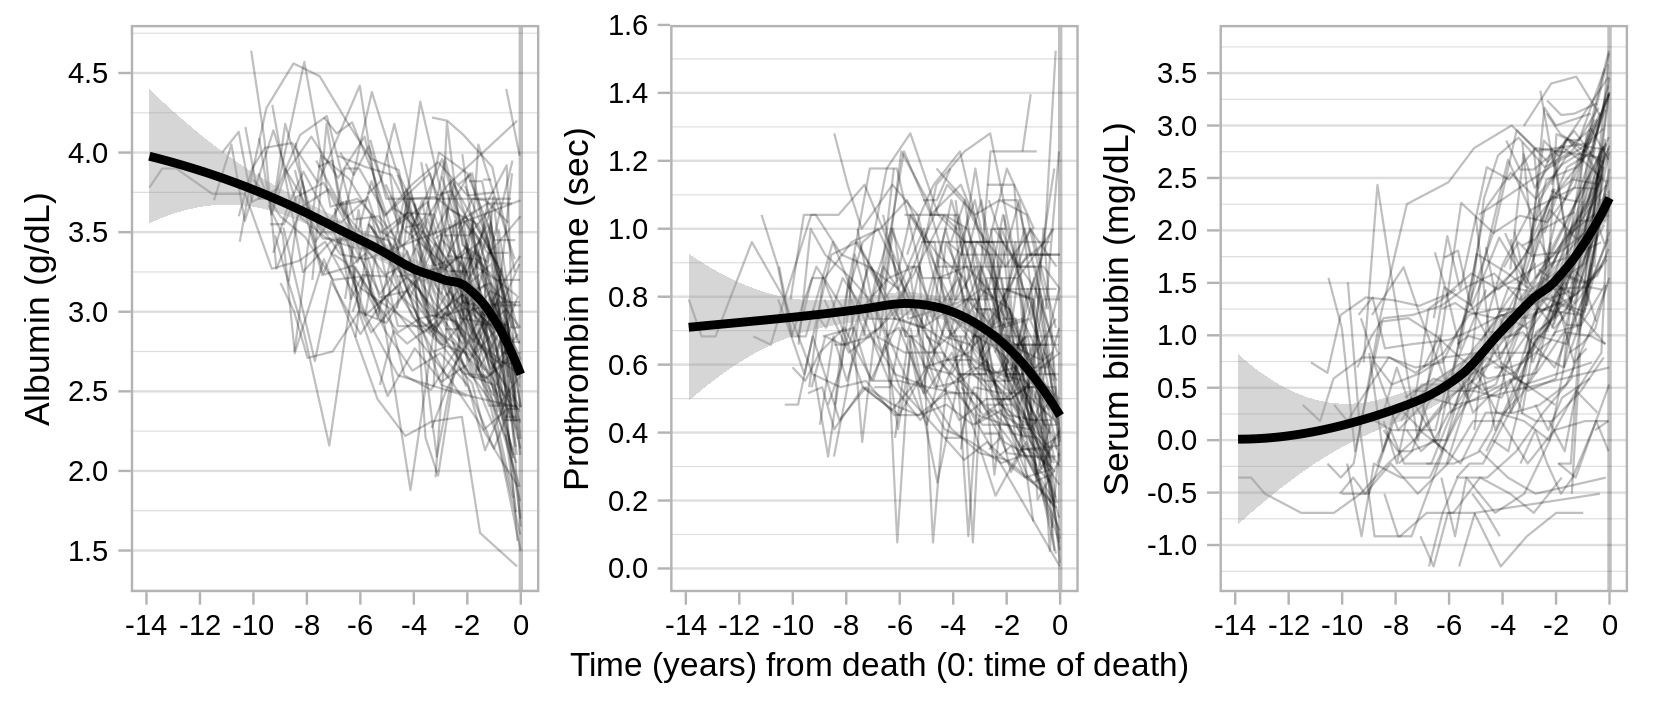
\includegraphics{Figures_Chapter1/PBCtrajectories.png}
      \caption{Longitudinal trajectories for three chosen biomarkers from PBC data. Grey lines show individual trajectories and overlaid smoothed (LOESS) curves the average trajectories for those who experienced mortality during follow-up and those who did not.}
      \label{fig:PBCtrajectories}
  \end{figure}
  
  %\resettocmain
  \section{Thesis outline}\label{sec:intro-thesis-outline}
  % One line introduction -->
  With an overview of joint modelling and its development in literature provided in Sections \ref{sec:jointintro} and \ref{sec:intro-evolution-parent}, we proceed by presenting the structure of the thesis on a chapter-by-chapter basis.
  
  % `Classic' methods -->
  In Chapter \ref{cha:methods-classic}, we lay the foundations for the thesis by first establishing the notation to be used throughout. We then introduce the multivariate extension of the `classic' joint models, which are our specific models of interest, elucidating parameters of interest as well as the estimation routine. Couched in a semiparametric maximum likelihood approach we provide an overview of the EM algorithm, aligning our methodology with  `classic' literature. Stemming from this approach, we introduce numerical integration methods. We further outline how one can `complete' inference and obtain standard errors for a fitted joint model. Finally, we offer a comprehensive overview of simulating data within the joint modeling framework; a crucial technique for the forthcoming chapters.
  
  % Approximation -->
  In Chapter \ref{cha:approx}, we draw attention to the computational burden which precludes, or makes overtly cumbersome, estimation for multivariate joint models by maximum likelihood. We introduce a normal approximation first proffered by \citet{Bernhardt15}, with details of this approximate EM algorithm provided; the approximation is used exhaustively throughout the thesis. Extensive simulation results are given, which serve to showcase the performance of the algorithm. Additionally, we offer comparison in terms of computation time as well as parameter estimates with existing software which is similar in its estimation approach.

  % GMVJM -->
  In Chapter \ref{cha:flexible} we continue utilising the approximate EM algorithm but extend the longitudinal sub-model to the non-Gaussian case; the idea being that many clinical data will not be continuous, or the Gaussian assumption not otherwise appropriate. We consider five different exponential families and provide an overview of the estimation procedure required for these so-called `generalised' multivariate joint models in a similar spirit to Chapter \ref{cha:approx}. Once more we provide multitudes of simulation study results to exhibit performance of the approximate EM algorithm.

  % Justification -->
  Owing to its large-scale use in the thesis it is of considerable importance to thoroughly investigate, understand, and justify the normal approximation. In Chapter \ref{cha:justification}, beginning with its foundations before delineating strategies to justify said approximation, we seek to achieve this; swathes of results are provided along with interpretation.

  % Post-hoc analyses -->
  We then shift focus to avenues for analysis of a fitted joint model. That is, with the methodology outlined in Chapters \ref{cha:methods-classic}--\ref{cha:flexible}, what can one \textit{do} with the fitted joint model: Does it fit the data well? How can it be used for predictions? Such questions are answered in Chapter \ref{cha:posthoc} where we collate post-hoc analyses, from defining residuals for the two processes, to outlining how one can bridge from a joint model to a predictive one.

  % PBC application -->
  Chapter \ref{cha:app-PBC} can be viewed as something of an amalgamation of Chapters \ref{cha:methods-classic}, \ref{cha:approx}, \ref{cha:flexible}, and \ref{cha:posthoc}. We seek to provide an extensive application to the motivating set of clinical data from Section \ref{sec:intro-motivation-pbc}: The aim of the chapter is to identify, and perform post-hoc analyses on, the `best-fitting' (multivariate) joint model for the data.  

  % Conclusions/Future work and appendices -->
  Finally, the thesis is brought to a close by our conclusions along with discussions of possible future research avenues in Chapter \ref{cha:conclusion}. The thesis is supplemented by Appendices \ref{cha:appendix-ExtraStuff}--\ref{cha:appendix-supplementary-figures} which house an assortment of extra derivations and results (both tabulated and graphical). Furthermore Appendix \ref{cha:appendix-gmvjoint} provides a brief overview of the \tt{R} package built alongside the work in Chapter \ref{cha:flexible}, \tt{gmvjoint} \citep{Murray2023}, which is used to obtain \textit{all results} presented in the thesis.
\end{chapter}